\documentclass[aspectratio=169]{beamer}
\usepackage{generic}
\begin{document}

\begin{frame}
  \title{\darkblue Introduction to the TAF package\\[1ex]
    \normalsize\darkgreen 2~ Running a TAF analysis}
  \author{\vspace{-16ex}\small\darkgray\it Arni Magnusson and Colin Millar}
  \date{}
  \titlepage
\end{frame}

% ______________________________________________________________________________

\begin{frame}{Overview}
  \begin{itemize}
    \item[] {\bf\darkblue 1~ Background} \comment{objectives, design}\\[3ex]
    \item[] {\bf\darkblue 2~ Running a TAF analysis} \comment{linear regression,
      boot and run, structured scripts}\\[3ex]
    \item[] {\bf\darkblue 3~ TAF features} \comment{boot procedure, data flow,
      new analysis, overview of functions}\\[3ex]
    \item[] {\bf\darkblue 4~ The TAF community} \comment{browsing an existing
      analysis, related R packages}\\[3ex]
    \item[] {\bf\darkblue 5~ Discussion} \comment{contents of a TAF analysis,
      benefits of TAF}\\[3ex]
    \item[] {\bf\darkblue 6~ Online examples} \comment{ICES, FAO, SPC,
      various}\\[3ex]
  \end{itemize}
\end{frame}

% ______________________________________________________________________________

\begin{frame}{Linear Regression Example}\small
  \begin{itemize}
    \item[] To demonstrate how a TAF analysis works, consider a simple linear
    regression\\[0.2ex]
    where the $x$ and $y$ coordinates come from a text file. The
    {\tt\green linreg} example\\[0.2ex]
    comes with the TAF package and can be copied to a convenient place to
    test\\[0.2ex]
    and run:\\[4ex]\tt
    \qquad{\blue library}(TAF)\\[0.5ex]
    \qquad{\blue taf.example}("linreg")\\[0.5ex]
    \qquad{\blue setwd}("linreg")
  \end{itemize}
\end{frame}

% ______________________________________________________________________________

\begin{frame}{Boot and Run}\small
  \begin{itemize}
    \item[] Before running the analysis, the workflow\\[0.2ex]
    consists of a boot folder and four TAF scripts:\\[2ex]
    \qquad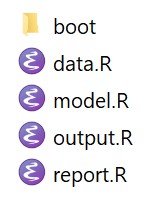
\includegraphics[width=0.12\textwidth]{explorer_1}
  \end{itemize}
\end{frame}

% ______________________________________________________________________________

\begin{frame}{Boot and Run}\small
  \begin{itemize}
    \item[] To run a TAF analysis, the first step is to start R and make sure
    that\\
    the {\green current working directory} is set to the location of the TAF
    scripts\\
    {\tt data.R}, {\tt model.R}, etc.\\[4ex]
    Some R editors do this automatically when opening an R script and\\
    in RStudio there is a menu command:\\[1ex]\it
    \qquad Session - Set Working Directory - To Source File Location\\[2ex]
    \green\sf\qquad[\:\!Alt-s w s\;\!]
  \end{itemize}
\end{frame}

% ______________________________________________________________________________

\begin{frame}{Boot and Run}\small
  \begin{itemize}
    \item[] All TAF analyses can be run using the following commands in
    R:\\[2ex]
    \begin{itemize}\tt\item[]
      {\blue library}(TAF)\\
      {\blue taf.boot}()\\
      {\blue source.all}()\\[3ex]
    \end{itemize}
    \item[] The {\tt\blue taf.boot()} function looks for an existing boot folder
    to set up the\\ data and software required for the analysis.\\[3ex]
    Then {\tt\blue source.all()} runs the {\tt data.R}, {\tt model.R}
    {\tt output.R}, and {\tt report.R}\\ scripts in that order.\\[3ex]
    The individual scripts can also be run using {\tt\blue source()} or line by
    line in an\\
    R editor.\\[4ex]
  \end{itemize}
\end{frame}

% ______________________________________________________________________________

\begin{frame}{Boot and Run}\small
  \begin{itemize}
    \item[] After running the analysis, each script has created a corresponding
    folder,\\[0.2ex]
    {\tt data.R} creating a data folder, etc.\\[4ex]
  \end{itemize}
  \centering
  \begin{columns}[T]
    \column{0.1\textwidth}
    \column{0.12\textwidth}
    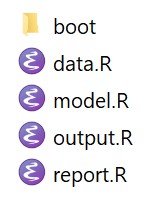
\includegraphics[width=\textwidth]{explorer_1}
    \column{0.06\textwidth}
    \vspace{7ex}
    \centering\darkgray\large$\Rightarrow$
    \column{0.12\textwidth}
    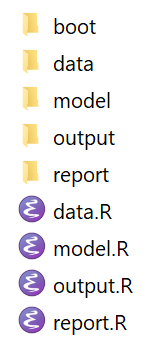
\includegraphics[width=\textwidth]{explorer_2}
    \column{0.3\textwidth}
  \end{columns}
\end{frame}

% ______________________________________________________________________________

\begin{frame}{Structured scripts}\small
  The {\tt\darkblue data.R} script has populated the {\tt data} folder with
  comma-separated\\
  values (CSV) files representing the
  {\green data that are used in the analysis} and the\\
  {\tt model.R} script produced model results in a machine-readable
  format.\\[3ex]

  The purpose of the {\tt\darkblue output.R} script is to
  {\green read the results} from the model\\
  folder and write out CSV files representing the results that are of primary
  interest.\\[3ex]

  Finally, {\tt\darkblue report.R} reads in the CSV output and produces
  {\green plots and formatted\\
    tables}, often with rounded numbers, which can be incorporated into a
  report.\\[3ex]

  The {\tt\darkblue report.R} script can also produce a
  {\green dynamic document} in various formats\\
  if the scientist writes the script in that way.\\[3ex]

  It is important to note that TAF does not do any of this by itself. All the
  work\\
  is performed by the R scripts that the scientist writes.\\[3ex]
\end{frame}

% ______________________________________________________________________________

\begin{frame}{Structured scripts}\small
  Typically, a TAF script has the following general structure:\\[3ex]\tt\fns
  \begin{itemize}\item[]
    \begin{gray}
      \# What the script does\\[1em]
      \# Before: file1.csv, file2.rds, file3.spec (previous)\\
      \# After:  file4.csv, file5.csv, file6.png (folder)\\[1em]
    \end{gray}
    {\blue library}(TAF)\\
    {\blue library}(SomePackage)\\
    {\blue source}("utilities.R")\\[1em]
    {\blue mkdir}("folder")\\[3ex]
  \end{itemize}
\end{frame}

% ______________________________________________________________________________

\begin{frame}{Structured scripts}\small
  \begin{itemize}\item[]\tt\fns
    {\gray \# Read files from previous step}\\
    dat1 <- {\blue read.taf}("previous/file1.csv")\\
    dat2 <- {\blue readRDS}("previous/file2.rds")\\
    dat3 <- {\blue importSpecial}("previous/file3.spec")\\[1em]
    {\gray \# Some computations}\\
    {\gray \# [...]}\\[1em]
    {\gray \# Write out tables and plots}\\
    {\blue write.taf}(dat4, dir="folder")\\
    {\blue write.taf}(dat5, dir="folder")\\
    {\blue taf.png}("file6")\\
    {\blue SpecialPlot}(dat6)\\
    {\blue dev.off}()\\[3ex]
  \end{itemize}
\end{frame}

% ______________________________________________________________________________

\begin{frame}{Summary}
  \begin{itemize}
    \item[] {\bf\darkblue 1~ Background} \comment{objectives, design}\\[3ex]
    \item[] {\bf\darkblue 2~ Running a TAF analysis} \comment{linear regression,
      boot and run, structured scripts}\\[3ex]
    \item[] {\bf\darkblue 3~ TAF features} \comment{boot procedure, data flow,
      new analysis, overview of functions}\\[3ex]
    \item[] {\bf\darkblue 4~ The TAF community} \comment{browsing an existing
      analysis, related R packages}\\[3ex]
    \item[] {\bf\darkblue 5~ Discussion} \comment{contents of a TAF analysis,
      benefits of TAF}\\[3ex]
    \item[] {\bf\darkblue 6~ Online examples} \comment{ICES, FAO, SPC,
      various}\\[3ex]
  \end{itemize}
\end{frame}

\end{document}
